In this section, we present the inference model to localize the failures based on the path level measurements. ~\ref{fig:example} shows a simple example network we target in this paper. It consists of a number of sites interconnected by a network cloud 
where only the network nodes and their interfaces are known (otherwise the failure localization is meaningless). 
A distributed application will incur traffic flows along an unknown path between pairs of end hosts. These flows are subject to 
the measurement of the applications to test if they are corrupted. Two such flows, $c3-d2$ and $c2-d4$ are shown in the figure. Intuitively, 
if both flows suffers from data corruption, the interface with the cross mark in Node $N2$ should be inferred to be the culprit.   

\begin{figure}
  \begin{center}
    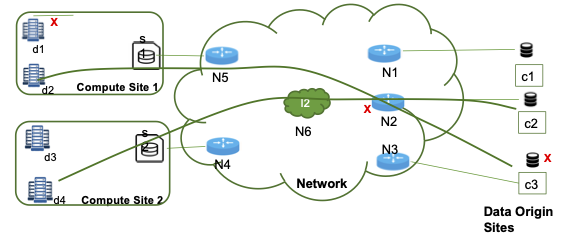
\includegraphics[width=0.48\textwidth]{./figure/example_network.png}
  \end{center}
\caption{An Example Network}
\label{fig:example}
\end{figure}

In most existing work on in gray failure localization , the network is modeled as a simple graph $G(V,E)$  
with a set of nodes $V$ connected by a set of links $E$. The following bipartite mapping 
formula was used to capture the relationship between the link failures and the path level measurements~\cite{netbouncer:nsdi18,DeepView:NSDI18,arzani2018democratically}. 
The failure being considered is packet loss. 
The reasonings behind these models are similar: due to scalability or privacy constraints, 
monitoring every component of interest in a large-scale network is 
not feasible, while the path level measurement is more practical to deploy and instrument.  
\begin{flalign}\label{eq:prob}
\begin{aligned}
&P(No\ Failure\ in\ Path \ i) = \\
&\prod_{j \in Path\ i}P(component\ j\ is\ normal)
\end{aligned}
\end{flalign}
This can be transformed to a familiar linear regression model for every identifiable path in the network after taking log on the equations.
\begin{flalign}\label{eq:linear}
\begin{aligned}
&p_i = &\sum_{j \in Path\ i} c_j\ & \forall i \in P
\end{aligned}
\end{flalign}
Here $P$ represents the set of paths that are measured and a fundamental assumption underscoring these models is that routing of every path 
in $P$ over link set $E$ need to be obtained. In addition, it was also assumed the measurement system have the access to all network nodes 
to instrument path measurements, \ie, the source and destination of a path can be any nodes. In summary, in order to 
establish the regression model to obtain satisfactory inference performance, 
substantial efforts were made to (i) identify the routing of the paths, (ii) determine the path set for good coverage, and 
(iii) enable constant measurement of paths. Then the path measurements ($p_i$) will be obtained to estimate the link error probability ($c_j$) using this model.

In our wide-area multi-domain network setting, as we discussed in an earlier work~\cite{iris:ictc21}, it is not practical to identify the routing of 
the paths over the network and even the network topology beforehand. This means that it is difficult to establish a model like Eq. (\ref{eq:linear}). 
We also can not assume the access to nodes in the network domains to instrument or measure paths.  

We thereafter distinguish between application end hosts (that generate and receive data) and networking devices (routers or switches), 
\ie, $V$ includes $H$ end hosts and $R$ routers. And we redefine $E$ to be the set of network components where failures are supposed to be 
localized, specifically all the network interfaces on $V$ and the end hosts $H$. We further constrain that only passive path measurements are available from certain applications on the end hosts, \ie, $P$ in our system only consists of paths originating from and ending in end hosts in $H$, which implies a much smaller identifiable path set. In the example network Fig.~\ref{fig:example}, none of the network nodes, $N1, \ldots, N6$, can be the source or destination of a path. And for a path between two end hosts, its routing is unknown. The only knowledge our model has is the bag of nodes and their interfaces for traffic forwarding.  

We further observe that one component failure (e.g., $x_j$) 
could cause multiple paths erroneous while one erroneous path may be the result of a failure at different components. The standard model Eq. (\ref{eq:linear}) actually ignores 
the correlation between multiple paths sharing a common component. We thereafter inverse the equations to represent the component failure probability as a function of 
the path failure probabilities as the following prediction model. 
 
\begin{flalign}\label{eq:inverse}
\begin{aligned}
Y = F(x_1, \cdots, x_p, \cdots, x_{|P|} ) \\
 = \sum_{p \in P} w_p x_p +w_0
\end{aligned}
\end{flalign}

Specifically, $Y$ represents a vector space $(y_1, \ldots, y_v, \ldots, y_{|V|)}$ where $y_v$ represents the failure probability of component 
$v \in V$.  $X = (x_1, \ldots, x_p, \ldots, x_{|P|})$  forms the feature space that is defined by the combinations of the path failure probability. 
As shown in Eq. (\ref{eq:inverse}), we can further make it a linear regression model, which gives excellent performance as we will show in 
the evaluation section. We note, unlike in the existing work where failure localization is on network links, the network components in our model 
are the nodes and their interfaces because we assume the network topology is unknown.

Since any component failure only affects a small number of paths that go through it, plus multiple simultaneous failures are rare in reality, it is 
reasonable to expect both the feature matrix and the coefficient matrix are sparse, representing the samples collected during one inference 
window. This suggests to use the regularization technique to make most of the estimated coefficient to be zero. The most efficient technique 
to achieve this intention is to add a L1-norm constraint is known as Lasso~\cite{DeepView:NSDI18}, where the regression optimization objective 
is defined as:    

\begin{flalign}\label{eq:lasso}
\begin{aligned}
\hat{W} =  \argmin_{W \in R^{|P|}}\vert\vert{\textbf{Y}-\textbf{X}W}\vert\vert _2^2 + \lambda \vert\vert{W}\vert\vert_1
\end{aligned}
\end{flalign}

Here $\textbf{Y}$ and $\textbf{X}$ are the sample matrix. This technique has proven extremely efficient in dealing with overfitting. 
The vector definition of $Y \in R^{|C|}$ means for each sample $n$, all entries but one in $Y^n$ are zeros. 
Comparing to the scalar variable of a specific component failure probability, this multi-output model 
captures the independence between all the failures and would help the training and prediction quality.  








